% Этот шаблон документа разработан в 2014 году
% Данилом Фёдоровых (danil@fedorovykh.ru) 
% для использования в курсе 
% <<Документы и презентации в \LaTeX>>, записанном НИУ ВШЭ
% для Coursera.org: http://coursera.org/course/latex .
% Исходная версия шаблона --- 
% https://www.writelatex.com/coursera/latex/5.1

\documentclass[t]{beamer}  % [t], [c], или [b] --- вертикальное выравнивание на слайдах (верх, центр, низ)
%\documentclass[handout]{beamer} % Раздаточный материал (на слайдах всё сразу)
%\documentclass[aspectratio=169]{beamer} % Соотношение сторон

%\usetheme{Berkeley} % Тема оформления
%\usetheme{Bergen}
%\usetheme{Szeged}

%\usecolortheme{beaver} % Цветовая схема
%\useinnertheme{circles}
%\useinnertheme{rectangles}

%%% Работа с русским языком
\usepackage{cmap}					% поиск в PDF
\usepackage{mathtext} 				% русские буквы в формулах
\usepackage[T2A]{fontenc}			% кодировка
\usepackage[utf8]{inputenc}			% кодировка исходного текста
\usepackage[english,russian]{babel}	% локализация и переносы

%% Beamer по-русски
\newtheorem{rtheorem}{Теорема}
\newtheorem{rproof}{Доказательство}
\newtheorem{rexample}{Пример}

%%% Дополнительная работа с математикой
\usepackage{amsmath,amsfonts,amssymb,amsthm,mathtools} % AMS
\usepackage{icomma} % "Умная" запятая: $0,2$ --- число, $0, 2$ --- перечисление

%% Свои команды
\DeclareMathOperator{\sgn}{\mathop{sgn}}

%% Перенос знаков в формулах (по Львовскому)
\newcommand*{\hm}[1]{#1\nobreak\discretionary{}
{\hbox{$\mathsurround=0pt #1$}}{}}

%%% Работа с картинками
\usepackage{graphicx}  % Для вставки рисунков
\graphicspath{{img/}}  % папки с картинками
\setlength\fboxsep{3pt} % Отступ рамки \fbox{} от рисунка
\setlength\fboxrule{1pt} % Толщина линий рамки \fbox{}
\usepackage{wrapfig} % Обтекание рисунков текстом

%%% Работа с таблицами
\usepackage{array,tabularx,tabulary,booktabs} % Дополнительная работа с таблицами
\usepackage{longtable}  % Длинные таблицы
\usepackage{multirow} % Слияние строк в таблице

%%% Программирование
\usepackage{etoolbox} % логические операторы

%%% Другие пакеты
\usepackage{lastpage} % Узнать, сколько всего страниц в документе.
\usepackage{soul} % Модификаторы начертания
\usepackage{csquotes} % Еще инструменты для ссылок
%\usepackage[style=authoryear,maxcitenames=2,backend=biber,sorting=nty]{biblatex}
\usepackage{multicol} % Несколько колонок

%%% Картинки
\usepackage{tikz} % Работа с графикой
\usepackage{pgfplots}
\usepackage{pgfplotstable}

\usetheme{Boadilla}
\usecolortheme{default} % Кого мы обманываем, она топовая :)

\title{Презентация ужина}
\subtitle{или как провести идеальный день рождения}
\author{Анатолий Бордиян}
\date{\today}
\institute{Конфетки, бараночки ltd.}

\begin{document}

\frame[plain]{\titlepage}	% Титульный слайд

\section{Закуски}
 
\begin{frame}
	\frametitle{\insertsection} 
	\framesubtitle{\insertsubsection}
	\begin{columns}
		\begin{column}[t]{0.5\linewidth}
			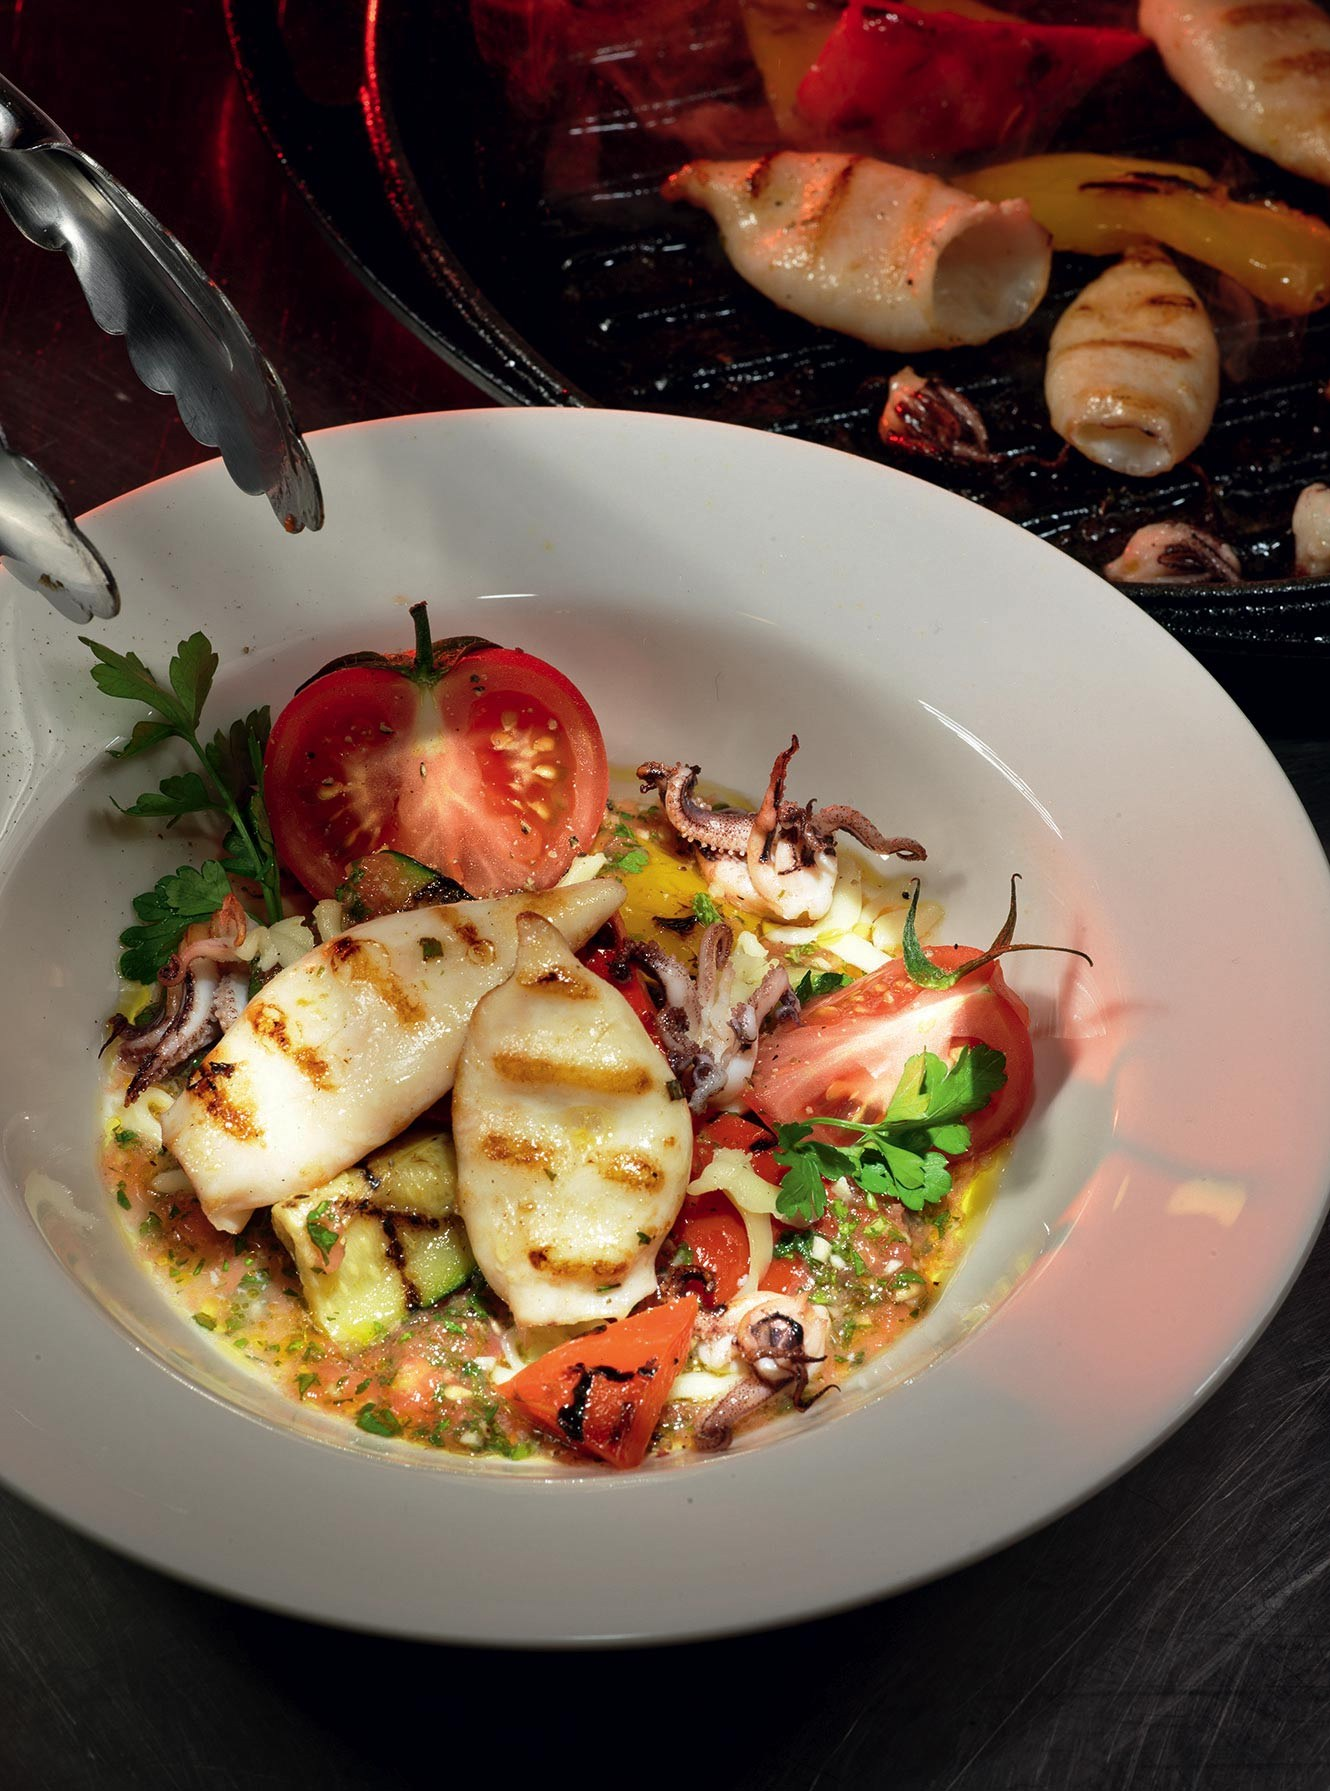
\includegraphics[height=5cm, width=4.5cm]{salad_with_squids.jpg}
			\begin{itemize}
				\item Салат с кальмарами
			\end{itemize}
		\end{column}	
	\pause	
		\begin{column}[t]{0.5\linewidth}
			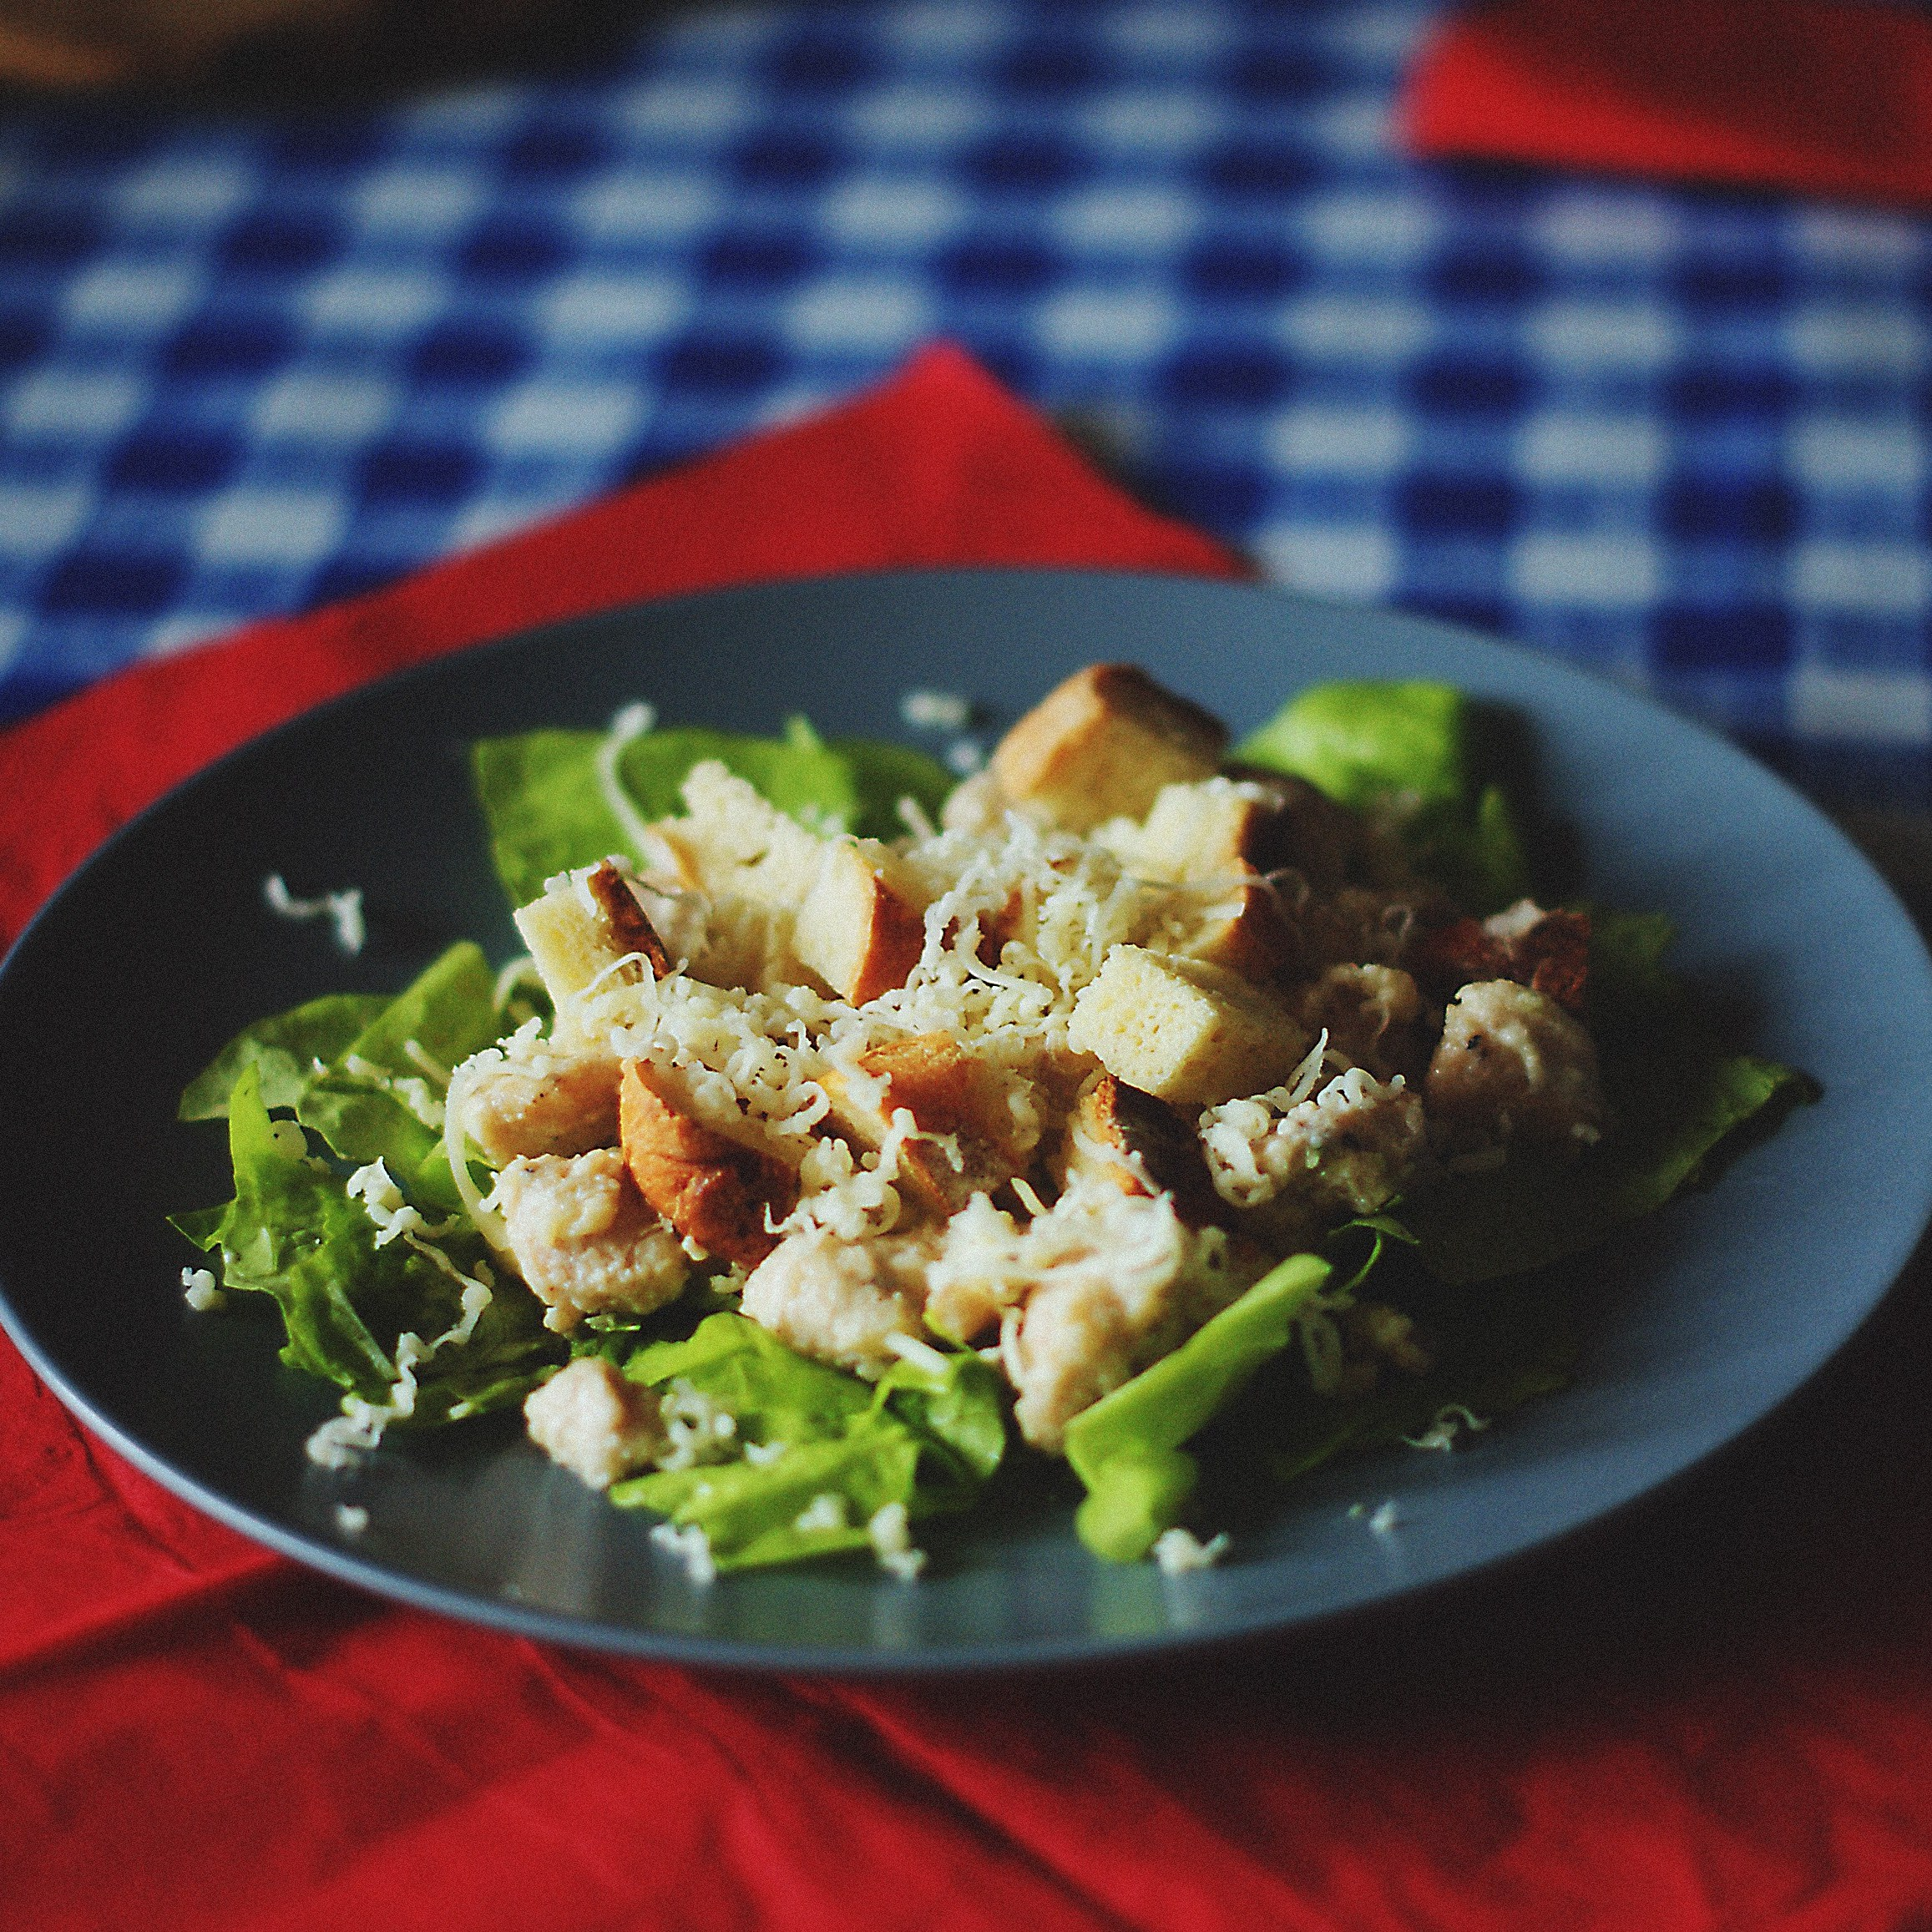
\includegraphics[height=5cm, width=4.5cm]{Cezar.jpg}
			\begin{itemize}
				\item Салат <<Цезарь>>
			\end{itemize}
		\end{column}
	\end{columns}
\end{frame}

\section{Развлечения}
{
\usebackgroundtemplate{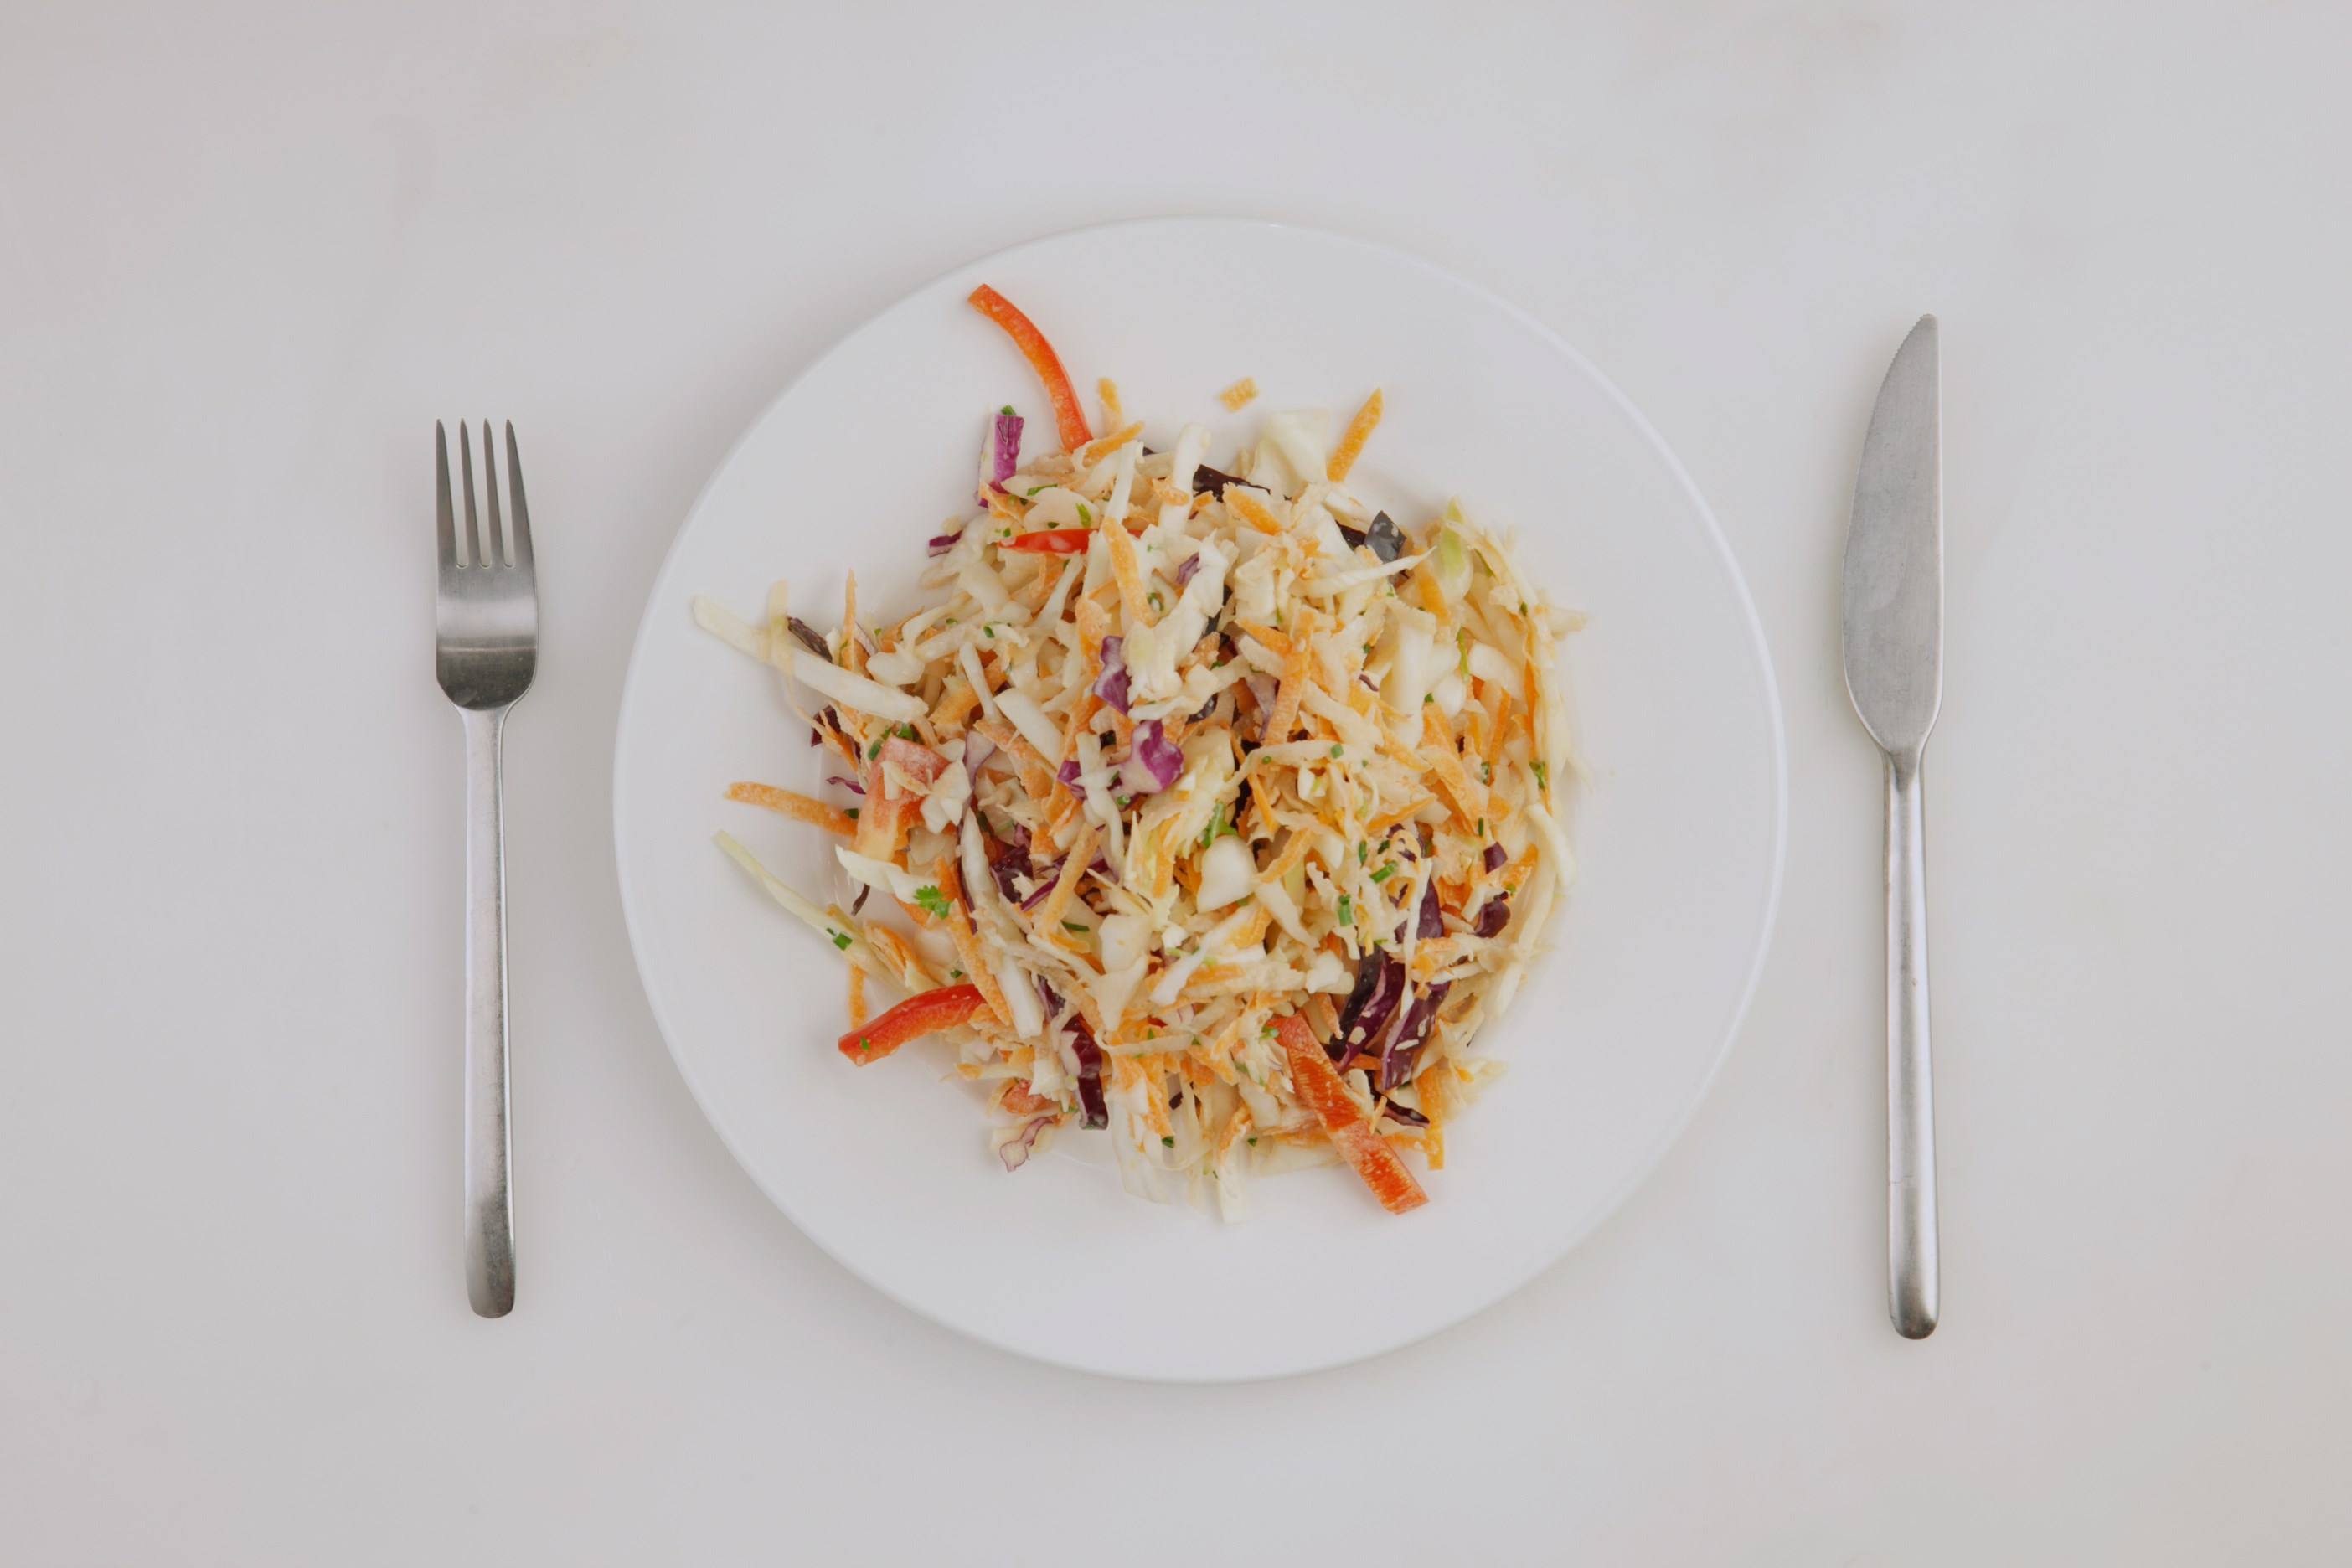
\includegraphics[width=\paperwidth,height=\paperheight]{Kouslo.jpg}}
\begin{frame}
	\frametitle{\insertsection}
	\framesubtitle{\insertsubsection}
	\begin{enumerate}
		\item<1> \href{https://oz.by/}{Настолки! (Купить можно здесь)}
		\item<2-3> Караоке.
		\item<3> И танцы.
		\item<4> Песни под гитару.
		\item<1-3> Веселье!!!
	\end{enumerate}
\end{frame}
}

\section{Основные блюда}
\begin{frame}
\frametitle{\insertsection}
\framesubtitle{\insertsubsection}
	\only<1>{ 
		\begin{block}{Картофель <<Айдахо>>}
			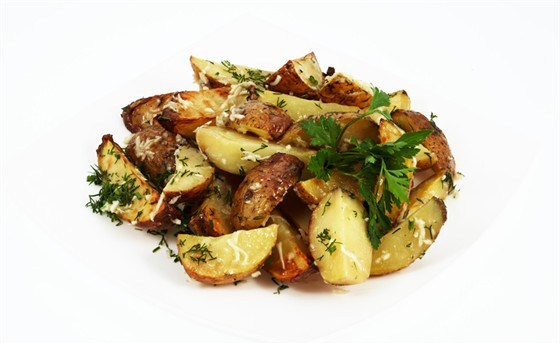
\includegraphics[height=7cm, width=10cm]{potato.jpg}
		\end{block}
	}
	\only<2>{ 			
		\begin{block}{Хек в зеленом чесночном соусе}
		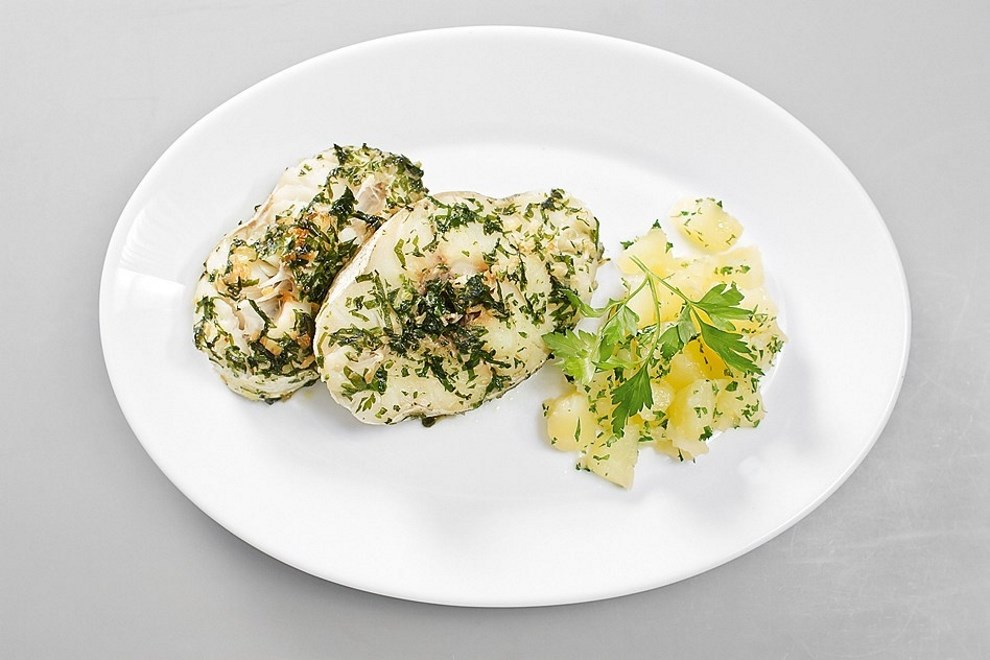
\includegraphics[height=7cm, width=10cm]{hek.jpg}
		\end{block}
	}
\end{frame}

{
\usebackgroundtemplate{
\includegraphics[width=\paperwidth,height=\paperheight]{tortik.jpg}}
\begin{frame}[plain,c]
	\begin{center}
		\alert{С днём рождения!}
	\end{center}
\end{frame}
}
\end{document}